\documentclass[final,3p,times,twocolumn]{elsarticle}

\usepackage[utf8]{inputenc}
\usepackage{xspace}
\newcommand{\spin}{SPIN\xspace}
\newcommand{\rev}[1]{#1}   % revision markup disabled for submission
\usepackage{amsmath,amssymb,amsthm}
\usepackage{url}
\usepackage{graphicx}
\usepackage{booktabs}
\usepackage{enumitem}
\usepackage{xcolor}
\newcommand{\fix}[1]{#1}  % round-2 corrections; set to \textcolor{red}{#1} to re-enable highlighting
\setlist[itemize]{itemsep=1pt, topsep=2pt, parsep=0pt, partopsep=0pt}

\newtheorem{proposition}{Proposition}
\newtheorem{lemma}{Lemma}
\newtheorem{assumption}{Assumption}
\newtheorem{remark}{Remark}
\newtheorem{definition}{Definition}

\journal{Journal of Process Control}

\begin{document}

\begin{frontmatter}

\title{Model-Free PID Tuning by Step-Response Inspection}

\author[inst1]{Daniel Pachner}
\author[inst1]{Pavel Otta\corref{cor1}}
\ead{pavel.otta@cvut.cz}
\author[inst1]{Ji\v{r}\'{\i} Dost\'al}
\author[inst2]{Vladim\'{\i}r Havlena}

\cortext[cor1]{Corresponding author}

\affiliation[inst1]{organization={University Centre for
Energy Efficient Buildings (UCEEB), Czech Technical University in
Prague}, city={Buštěhrad}, country={Czech Republic}}
\affiliation[inst2]{organization={Department of Control Engineering,
Faculty of Electrical Engineering, Czech Technical University in Prague},
city={Prague}, country={Czech Republic}}

\begin{abstract}
Industrial PID loops are still tuned by hand: the engineer steps the
setpoint, looks at the response, and changes a gain. This paper turns
that procedure into an algorithm. From a single closed-loop step
response we form three phase portraits of the control error and count
the winding number of each. The count is a scale-free, topological
diagnostic: independent of time and amplitude, it shows in which
frequency band the loop is under-damped---that of the integral, the
proportional, or the derivative channel. A triangular rule reads the
three counts, reduces the gain of the single band whose fault is
certain, and raises every band already measured within limits. No model is identified and no
optimization is solved. The deterministic iteration provably converges to the boundary of the
well-damped tuning set---the largest gains those limits allow---safely
on a running process and from arbitrary starting gains, including
destabilizing ones. The method assumes a stable, self-regulating
process with monotone gain and phase\fix{---first-order-plus-time-delay
models and higher-order lag chains with dead time among them---}and
a controller from the nested
family $\mathrm{I} \subset \mathrm{PI} \subset \mathrm{PID}$ with
integral action present. We validate it with
one fixed step size and one set of dimensionless constants, unchanged,
on a battery of process-typical plants. Every decision is visible: an
operator watching the portraits sees what the algorithm sees. We call
the method \spin, for Step-response Phase-portrait INspection; a
reference implementation and an interactive demonstration are public.
\end{abstract}

\begin{keyword}
PID control \sep controller tuning \sep data-driven control \sep
phase plane \sep step response
\end{keyword}

\end{frontmatter}

%=====================================================================
\section{Introduction}
%=====================================================================

Eighty years after Ziegler and Nichols \cite{ZN1942}, PID remains the
dominant industrial controller \cite{AstromHagglund2001}; a survey of
eleven thousand loops confirms this \cite{Desborough2002}. Most PID
loops are still tuned by inspection: an engineer steps the setpoint,
looks at the response, and adjusts a gain by judgment.

The literature offers three remedies, and all discard the inspection.
1)~Model-based rules---Ziegler--Nichols \cite{ZN1942}, Cohen--Coon
\cite{CohenCoon1953}, IMC \cite{RiveraIMC}, SIMC
\cite{Skogestad2003}---replace it with an identified low-order model,
and therefore inherit the errors of that model; both experimental parts
of Ziegler--Nichols have since been revisited with modern robustness
tools \cite{AstromHagglund2004,Schlegel2002}, the latter using a
value-set process description later formalized in
\cite{SchlegelCech2005}.
2)~Data-driven schemes replace the inspection with a criterion and the
machinery to serve it: a dedicated relay experiment
\cite{AstromHagglund1984}, gradient experiments on a quadratic cost
\cite{HjalmarssonIFT}, an identification-like problem \cite{CampiVRFT},
online perturbation of the gains
\cite{KillingsworthKrstic}.
\fix{3)~Parametric-region methods compute the admissible set directly in the
controller's parameter plane, every setting meeting an $H_\infty$
specification \cite{BrabecSchlegel2023,Ho2003}: a region with a certificate
rather than one tuning, but needing a plant model, a weighting function and a
level $\gamma$ fixed in advance, for two free parameters at a time.}

The closest precedent automated the inspection but did not formalize
it. The pattern-recognition autotuner of \cite{KrausMyron1984},
deployed industrially as EXACT, reads overshoot and decay ratio from
detected peaks of the transient and adjusts the gains by heuristic
logic. The inspection itself has never been made a well-defined
quantity: which gain is at fault, given this response, computed rather
than matched to a pattern.

The inspection differs from both families in the kind of quantity it
reads. Every diagnostic named above is metric---a ratio of amplitudes,
an integrated cost, an identified parameter with units---and therefore
needs a scale supplied for every loop by a model, a normalization, or
an expert. The turn index is topological instead: a property of
the oriented shape of the error trajectory, namely how many times it
wraps around its settling point, independent of units, amplitude, the
clock, and, in the fast-sampling limit, the sampling period
(Proposition~\ref{prop:invariance}). This is why the manual procedure
is blind to scale, and why one fixed set of dimensionless thresholds
serves every plant in this paper.

This paper formalizes the inspection. We call the resulting method
\spin, for Step-response Phase-portrait INspection. The contributions
are the following. (i)~A triple of phase portraits of the control error whose
turn indices form a dimensionless, scale-free, band-selective,
topological damping diagnostic (Section~\ref{sec:index}).
(ii)~A well-posedness analysis of the index. It includes a
counterexample in which a naively windowed count diverges, and a
settling-anchored guard that restores window independence
(Section~\ref{sec:wellposed}). (iii)~A single triangular tuning rule in
band-ordered gain coordinates, read as band-wise loop shaping.
Boundedness holds unconditionally, and convergence to the boundary
follows from a monotonicity property derived from the plant class
(Proposition~\ref{prop:mono}, Section~\ref{sec:rule}).
(iv)~Validation on a battery of process-typical plants with the same
default parameters throughout (Section~\ref{sec:battery}).

\rev{The paper introduces the method, and its setting is deliberately
the simplest one in which every mechanism is visible: the analysis is
noise-free, the step size is a fixed default, and no acceleration or
step-size adaptation is attempted. These choices are not limitations of
the idea but of this presentation---a fixed step is also what runs
safely on a plant. Noise, adaptive steps, and the asymptotic behavior
of the iteration are natural continuations and are left to subsequent
work.}

The method claims no optimality. It returns a fast, well-damped
tuning, which is what an expert tuner also offers, and it asks for one
closed-loop setpoint step per iteration and nothing else. There is no
model, no relay experiment, and no solver. The procedure is also fully
auditable, because an operator who watches the three plots sees exactly
what the algorithm sees. The whole method is governed by the fixed
dimensionless defaults of Table~\ref{tab:defaults}, and none of them
was adjusted for any plant.

Every move either repairs a diagnosed fault or, when no band objects,
raises all gains by one verified step. No iterate is an exploration
step, so the tuner runs safely on a process in operation---where
adaptive and learning-based tuners must perturb or run unchecked
controllers to acquire information
\cite{HjalmarssonIFT,KillingsworthKrstic}, here the information is a
by-product of a routine setpoint step under the current controller.
Figures~\ref{fig:init_step}--\ref{fig:tuned_portraits} show the method
on one plant (P2, Section~\ref{sec:battery}), starting from a severely
mis-tuned controller and shown before any mathematics: the response and
the portraits before and after tuning, recorded from the running
implementation (Data availability). This demonstration run starts from
unit gains $(K_p, K_i, K_d) = (1, 1, 1)$, the default configuration of
the interactive demonstration, with the derivative taken on the
measurement (Remark~\ref{rem:velocity}); pressing \emph{Tune} on the
P2 preset reproduces every number in
Figures~\ref{fig:init_step}--\ref{fig:tuned_portraits} and
\ref{fig:limitcycle}.

\begin{figure*}[t]
\centering
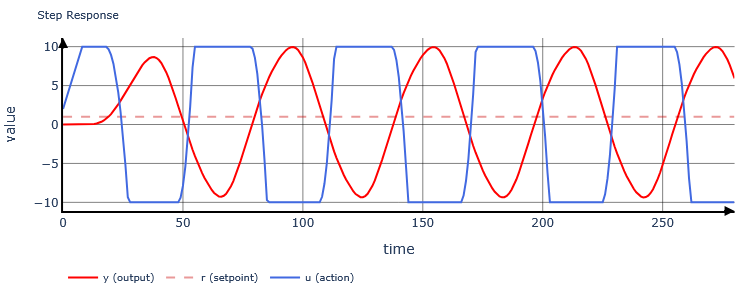
\includegraphics[width=0.70\textwidth]{init_step.png}
\caption{Step response before tuning (P2, unit gains). The mis-tuned
loop sustains an oscillation, and the actuator swings between its
limits. Nothing in this plot indicates which gain is at fault.}
\label{fig:init_step}
\end{figure*}

\begin{figure*}[t]
\centering
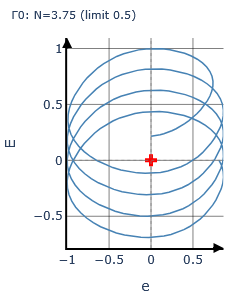
\includegraphics[width=0.32\textwidth]{init_F0.png}\hfill
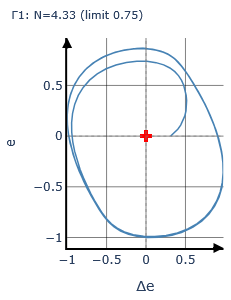
\includegraphics[width=0.32\textwidth]{init_F1.png}\hfill
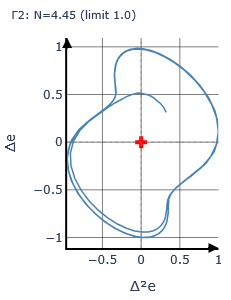
\includegraphics[width=0.32\textwidth]{init_F2.png}
\caption{Portraits before tuning, left to right
$\Gamma_0,\Gamma_1,\Gamma_2$; the cross marks the settling point. All
three counts are far above their limits ($N_0{=}3.75$ vs.\ $0.5$;
$N_1{=}4.33$ vs.\ $0.75$; $N_2{=}4.45$ vs.\ $1.0$). Which gain is at
fault cannot be read from Figure~\ref{fig:init_step}, but here the
violation is explicit in every band at once.}
\label{fig:init_portraits}
\end{figure*}

\begin{figure*}[t]
\centering

\includegraphics[width=0.70\textwidth]{tuned_step.png}
\caption{Step response after tuning: a single overshoot settling
cleanly to the setpoint, actuator unsaturated.}
\label{fig:tuned_step}
\end{figure*}

\begin{figure*}[t]
\centering
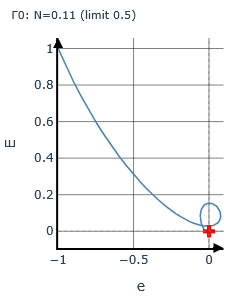
\includegraphics[width=0.32\textwidth]{tuned_F0.png}\hfill
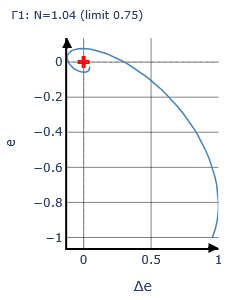
\includegraphics[width=0.32\textwidth]{tuned_F1.png}\hfill

\includegraphics[width=0.32\textwidth]{tuned_F2.png}
\caption{Portraits at the end of the run, one phase of the terminal
cycle. All three counts have fallen sharply from
Figure~\ref{fig:init_portraits}: $\Gamma_0$ is well within its limit
($3.75 \to 0.11$ vs.\ $0.5$), while $\Gamma_1$ and $\Gamma_2$
($4.33 \to 1.04$ vs.\ $0.75$; $4.45 \to 1.14$ vs.\ $1.0$) retain one
marginal lobe that a single gain notch removes and the next expanding
move re-creates. This is the boundary limit cycle of
Proposition~\ref{prop:conv} captured from its violated side, not a
failure to converge; the response at these gains is that of
Figure~\ref{fig:tuned_step}.}
\label{fig:tuned_portraits}
\end{figure*}

%=====================================================================
\section{The turn index}
\label{sec:index}
%=====================================================================

The method rests on exactly two standing assumptions, stated once and
used throughout.

\begin{assumption}[Process class]\label{ass:plant}
\fix{The plant $G$ is SISO, asymptotically stable and non-integrating
(self-regulating), and on $(0,\infty)$ both $|G(j\omega)|$ and $\arg G(j\omega)$ decrease
strictly, with $\arg G$ falling below $-3\pi/2$.}
\end{assumption}

\fix{Every clause is used: stability by the Nyquist step of
Proposition~\ref{prop:pair} and the backoff of
Remark~\ref{rem:bootstrap}, $|G(0)|<\infty$ by the sign in
Proposition~\ref{prop:mono}(i), monotone phase and gain by
Propositions~\ref{prop:pair} and~\ref{prop:band}, and the phase
condition to place the stability boundary at a finite gain, since
$\arg C \le \pi/2$ throughout Assumption~\ref{ass:pid}.}

\fix{For the class that covers most regulatory loops, membership is decidable
by inspection.}
\begin{lemma}[Lag chains with dead time]\label{lem:class}
Let $G(s) = K\,e^{-Ls}\prod_{i=1}^{n}(\tau_i s+1)^{-1}$ with $K>0$,
$\tau_i>0$, $L\ge 0$. Then $|G|$ and $\arg G$ decrease strictly on
$(0,\infty)$, and $\arg G$ falls below $-3\pi/2$ iff $L>0$, or $L=0$ and
$n\ge 4$; such a plant satisfies Assumption~\ref{ass:plant} exactly when
$L>0$ or $n\ge 4$.
\end{lemma}

\begin{proof}
Differentiating, $\mathrm d\log|G|/\mathrm d\omega =
-\sum_i \tau_i^{2}\omega/(1+\tau_i^{2}\omega^{2})$ and
$\mathrm d(\arg G)/\mathrm d\omega =
-L-\sum_i \tau_i/(1+\tau_i^{2}\omega^{2})$, both sums of strictly negative
terms for $\omega>0$. As $\omega\to\infty$, $\arg G \sim -L\omega - n\pi/2$:
for $L>0$ this diverges and $-3\pi/2$ is crossed, while for $L=0$ each
$\arctan$ approaches $\pi/2$ from below, so $-n\pi/2$ is never attained and
$n\ge4$ is required. Stability and $|G(0)|<\infty$ follow from $\tau_i>0$.
\end{proof}

\fix{So FOPTD and SOPTD models qualify for every $L>0$ and delay-free lag
chains from four lags up; in the batch of \cite{AstromHagglund2004} the
delay-free members of relative degree three sit on the $-3\pi/2$ limit, which
any dead time restores. Three classes fall outside: complex pole pairs damped
below $1/\sqrt2$, which show a gain peak; integrating plants, which also
reverse the sign in Proposition~\ref{prop:mono}(i); and plants with finite
zeros, whose rising magnitude the poles must dominate.
Assumption~\ref{ass:plant} stays readable from a measured frequency response
\cite{SchlegelCech2005,Schlegel2002}, Lemma~\ref{lem:class} being the shortcut
when a parametric form is known.}

\begin{assumption}[Controller structure]\label{ass:pid}
The controller is drawn from the nested family
$\mathrm{I} \subset \mathrm{PI} \subset \mathrm{PID}$: a parallel
structure $u = K_p e + K_i\!\int\! e + K_d \dot e$ in a unity-feedback
loop, with the integral channel mandatory ($K_i > 0$) and the
proportional and derivative channels optional ($K_p, K_d \ge 0$).
\end{assumption}

Write $C(s) = K_p + K_i/s + K_d s$ for the transfer function of the
controller of Assumption~\ref{ass:pid}.
Write $\theta = (K_p, K_i, K_d)$ for the controller's gains; a
uniform multiplier $m>0$ scales $\theta \mapsto m\theta$, an analysis
direction distinct from the per-band multipliers $(F_i, F_p, F_d)$ of
the rule (Section~\ref{sec:rule}). $C$ is linear in its gains, so
scaling all three by $m$ maps the loop $CG$ to $m\,CG$: the Nyquist
locus changes in magnitude but not in shape. A plant with an integrator
would satisfy the two monotonicity hypotheses yet reverse the sign in
Proposition~\ref{prop:mono}(i)---reducing all gains would destabilize
rather than damp, removing also the basis of
Remark~\ref{rem:bootstrap}; the \fix{non-integrating clause of
Assumption~\ref{ass:plant}} excludes this case.

A tuning experiment applies a setpoint step and
records the error $e_k$, $k = 0,\dots,K$, at period $T_s$, over a window
in which the response settles. Form the running integral $E_k$ and the
differences $\Delta e_k$, $\Delta^2 e_k$, and pair each signal with its
own difference:
\begin{align}
\Gamma_0&: \bigl(e_k,\, E_k{-}E_{K}\bigr), \notag\\
\Gamma_1&: \bigl(\Delta e_k,\, e_k\bigr), \notag\\
\Gamma_2&: \bigl(\Delta^2 e_k,\, \Delta e_k\bigr).
\label{eq:plots}
\end{align}
$\Gamma_1$ is the classical error phase plane. It is the
$(e,\dot e)$ portrait that has long been used to read nonlinear servo
transients graphically, with the shape of the trajectory taking the
place of a time history \cite{GrahamMcRuer1961}. The portraits
$\Gamma_0$ and $\Gamma_2$ are its integrated and differentiated
versions. All three end at the origin when the loop settles. We call
\eqref{eq:plots} \emph{Pachner plots}, after the first author, who
devised the construction.

A well-damped loop spirals into the origin without completing a full
turn, whereas an under-damped loop encircles it. The count is made precise as follows.

\begin{definition}[Turn index]\label{def:index}
Given a planar trajectory $(x_k, y_k)$, $k = 0,\dots,J$:
(i) normalize each coordinate by its peak magnitude, mapping the curve
into $[-1,1]^2$;
(ii) truncate at the last entry into the disc of radius
$\varepsilon \in (0,1)$ about the origin\fix{, retaining the curve in
full if it never enters that disc};
(iii) define $N$ as the winding number of the remaining curve about the
origin: total swept angle over $2\pi$, evaluated as the endpoint angle
difference corrected by signed crossings of the negative horizontal
semi-axis. Partial revolutions count fractionally.
\rev{If the curve never leaves the disc, $N := 0$.}
\end{definition}

Because $N$ is the winding number of the curve about the point at which
the loop settles, we call it the \emph{turn index}.

Definition~\ref{def:index} assumes that the trajectory ends at the
origin, and the integral channel guarantees this, since $e \to 0$ for
every stable tuning of Assumption~\ref{ass:pid}. Without integral
action the situation changes. A loop with proportional action only, on
a self-regulating plant, settles at a nonzero offset. Then $\Gamma_0$
and $\Gamma_1$ end away from the origin, the truncation of
Definition~\ref{def:index} never occurs, and the winding number
measures the wrong quantity. This is what the requirement $K_i > 0$
means in practice.

Applying Definition~\ref{def:index} to $\Gamma_0, \Gamma_1, \Gamma_2$
yields the turn-index vector $\mathbf N(\theta) = (N_0, N_1, N_2)$ at
controller setting $\theta = (K_p, K_i, K_d)$, from a single step test,
with no plant knowledge.

Four propositions carry the construction. The count is free of scale
and clock (Proposition~\ref{prop:invariance}); one damping dominates
the record, because stability is lost through one critical pole pair
(Proposition~\ref{prop:pair}); the count follows that damping, because
near the boundary the trajectory is a logarithmic spiral
(Proposition~\ref{prop:law}); and each portrait isolates one frequency
band, because each differencing tilts the spectrum by one power of
$\omega$ (Proposition~\ref{prop:band}).

\begin{proposition}[Topological invariance]\label{prop:invariance}
$\mathbf N$ is invariant under time reparametrization $t \mapsto \alpha t$,
$\alpha > 0$, of the underlying response, and under independent positive
scaling of either coordinate of each trajectory---in particular under
scaling of the setpoint step and, in the fast-sampling limit, of the
sampling period.
\end{proposition}

\begin{proof}
The winding number depends only on the oriented image of the curve, not
its parametrization; per-axis peak normalization removes amplitude and
units, and the truncation disc is defined on normalized coordinates.
\end{proof}

\begin{sloppypar}
One set of thresholds therefore serves all loops. The defaults
$\bar{\mathbf N} = (0.5, 0.75, 1.0)$, together with $\varepsilon = 0.1$,
are used unchanged in every result of this paper. They act as the
definition of ``well-damped'', not as adjustable settings. Since $N$
measures turns, the three limits are $2$, $3$ and $4$ quarter turns, so
each band is one quarter turn more tolerant than the band below it.
\end{sloppypar}

Which damping the counts read, and why a single damping dominates,
follows from the plant class.

\begin{proposition}[Critical pair]\label{prop:pair}
Let $G$ satisfy Assumption~\ref{ass:plant} and scale all
gains together, $CG \mapsto m\,CG$, $m>0$. The loop is stable up to a finite $m^\ast$ and loses stability there
through one complex pole pair, at the phase-crossover frequency
$\omega_{180}$, which maximizes $|CG(j\omega)|$ over
$\{\omega:\arg CG(j\omega)\rev{\equiv-\pi \pmod{2\pi}}\}$. Near
$m^\ast$ this pair is the least damped in the loop, and its damping
$\zeta(m)$ decreases continuously to zero as $m\uparrow m^\ast$.
\end{proposition}

\begin{proof}
$\Re\,C(j\omega) = K_p \ge 0$ bounds $\arg C$ to
$[-\pi/2,\pi/2]$, while \fix{$\arg G$ falls below $-3\pi/2$
(Assumption~\ref{ass:plant})}, so $\arg CG$ reaches
$-\pi$ at frequencies bounded away from $0$ and $\infty$. Increasing $m$ scales the locus $m\,CG$ radially, and by the Nyquist
criterion \cite{Nyquist1932} it first touches $-1$ at
$m^\ast = 1/|CG(j\omega_{180})|$, generically at one frequency.
The touch is transversal, since
$\partial|m\,CG|/\partial m = |CG| > 0$. One conjugate pair therefore
crosses the imaginary axis at $\omega_{180}$, while all other poles keep
strictly positive damping nearby. \rev{The transversal crossing gives
the strict decrease of $\zeta(m)$ near $m^\ast$, and continuity gives
$\zeta(m) \to 0$.}
\end{proof}

\rev{The mod-$2\pi$ formulation matters for strong derivative action:
with an unfiltered derivative on a dead-time plant $|CG|$ need not roll
off, and the first touch of $-1$ can fall on a later phase branch---the
fast branches of Remark~\ref{rem:scope}. Any derivative filter restores
the roll-off and keeps it on the first.}

Near the boundary a single pole pair therefore carries the ringing, and
we write
\begin{equation}
e(t) = A\,e^{-\alpha t}\cos(\omega t+\varphi) + r(t),
\qquad \zeta = \frac{\alpha}{\sqrt{\alpha^2+\omega^2}},
\label{eq:mode}
\end{equation}
where $r$ is the remaining, faster-settling part of the error. \fix{The
mode comes to dominate the record as $m \uparrow m^\ast$, since its
damping tends to zero while $r$ keeps its decay rate; the decomposition
is asymptotic in this sense rather than exact.} Between the
well-damped boundary and the stability boundary, which is where the
rule operates, it serves as the working model, and
Section~\ref{sec:battery} validates it. The propositions below are
based on \eqref{eq:mode}.

\begin{proposition}[Damping law]\label{prop:law}
For the mode of \eqref{eq:mode}, each truncated portrait of
Definition~\ref{def:index} winds
\begin{equation}
N = \frac{\ln(1/\varepsilon)}{2\pi}\,
\frac{\sqrt{1-\zeta^2}}{\zeta} + \eta,
\qquad |\eta| < 1,
\label{eq:law}
\end{equation}
where $\eta$ is a fractional endpoint term. The leading term
is strictly decreasing on $(0,1)$\rev{. The measured $N_k(\zeta)$
follows it within the band $|\eta|<1$---the truncation index makes
$\eta$, and hence $N_k$, piecewise constant with unit jumps---so each
threshold crossing $N_k=\bar N_k$ is localized to a damping interval,
and we take its midpoint as the calibrated damping $\bar\zeta_k$}.
\end{proposition}

\begin{proof}
Differentiation multiplies the mode by the fixed complex number
$-\alpha+j\omega$, so each portrait is a fixed linear image of the
mode's phase plane; a linear isomorphism preserves oriented loops, and
all three portraits trace one logarithmic spiral up to linear
equivalence. From its peak to the last entry into the
$\varepsilon$-disc the spiral's radius contracts by $\varepsilon$,
taking time $\alpha^{-1}\ln(1/\varepsilon)$, i.e.\
$(\ln(1/\varepsilon)/2\pi)(\omega/\alpha)$ revolutions, and
$\omega/\alpha=\sqrt{1-\zeta^2}/\zeta$; the truncated endpoints
contribute less than a half-turn each. Monotonicity:
$\mathrm d(\sqrt{1-\zeta^2}/\zeta)/\mathrm d\zeta<0$ on
$(0,1)$.
\end{proof}

It follows that\rev{, up to the endpoint band,}
$N_k>\bar N_k \iff \zeta<\bar\zeta_k$. The verdict
``rings'' is therefore a sign test, free of scale and of clock by
Proposition~\ref{prop:invariance}. The rule uses only this sign, but
inverting \eqref{eq:law} also gives a damping estimate at no extra
cost. Sampling shifts the constant in \eqref{eq:law}, most strongly in
$\Gamma_2$, but it never changes the monotonicity. The damping
specifications are therefore \emph{calibrated} rather than derived: for
the exact second-order step error, the measured $N_k(\zeta)$ crosses
$\bar{\mathbf N}=(0.5,0.75,1.0)$ at
$\bar\zeta \approx 0.64,\,0.49,\,\fix{0.34}$ with $\varepsilon=0.1$, which
is strictest in the lowest band. For a clean dominant mode the count is
set by $\varepsilon$, and the settling window of
Section~\ref{sec:wellposed} only guards against tails dominated by
noise.

Classical damping indicators read the same record differently:
overshoot needs a peak and a settled baseline, decay ratio and
logarithmic decrement need two peaks and a single mode, a damping ratio
needs a fitted model. The count $N$ needs none of these and, under
\eqref{eq:mode}, agrees with all of them, since all are monotone in
$\zeta$; only $N$, however, comes in three band-selective copies that
locate the oscillation in frequency, which is what the rule needs and
what separates it from pattern-recognition autotuning
\cite{KrausMyron1984}.

\begin{proposition}[Band selectivity and upward leakage]\label{prop:band}
Write $e = x + r$ as in \eqref{eq:mode}\rev{, with the residual $r$
essentially monotone with decay rate $\alpha_r<\omega_n=
\sqrt{\alpha^2+\omega^2}$. Then the visibility of the mode in
$\Gamma_j$ grows by the factor $\omega_n/\alpha_r>1$ per band number:
the mode is suppressed in every band below its own, and its visibility
increases monotonically from its own band upward. \fix{Its own band is
therefore the lowest one whose count it lifts, and} the set of bands
whose count a mode lifts is upward-closed, $\{k,k{+}1,\dots\}$}.
\end{proposition}

\rev{\begin{proof}
Each differencing step multiplies the mode by $\omega_n$ and the
residual only by $\alpha_r$, because monotonicity bounds the spectral
content of the residual below $\omega_n$; each integration does the
reverse. One band step therefore changes the mode-to-residual ratio by
$\omega_n/\alpha_r$. Several modes superpose, each contributing an
upward-closed set; interference between modes is neglected here, and the
synthetic tests below and Section~\ref{sec:battery} bear the
approximation out.
\end{proof}}

Each band belongs to one controller channel. For the parallel PID,
$|C(j\omega)| \approx K_i/\omega$ at low frequency, $\approx K_p$ in the
middle band, and $\approx K_d\omega$ at high frequency. Therefore $N_0$
points to $K_i$, $N_1$ points to $K_p$, and $N_2$ points to $K_d$. This
correspondence is the entire basis of the tuning rule.
\fix{It is assumed, not a consequence of
Proposition~\ref{prop:band}, which orders the portraits but does not
attach one to a controller channel. It presupposes that $K_i/K_p$ and
$K_p/K_d$ are separated; where $T_i \approx T_d$ the middle band does
not exist and $N_1$ loses selectivity.}

\emph{Attribution.} The violated set is a union of upward-closed sets
(Proposition~\ref{prop:band}). Its lowest member is therefore the only
band whose violation cannot be leakage, because no band below it exists
from which leakage could come. Violations above it carry no evidence
either way, since a genuine upper-band mode and upward leakage produce
counts that cannot be distinguished. In a synthetic test, one
under-damped middle mode alone gives
$\mathbf N = (0.12,\, 3.9,\, 6.5)$, where the high count exceeds the
middle one purely by leakage. A single high mode alone gives
$(0.12,\, 0.05,\, 5.7)$, and it leaks into no band below. The rule of
Section~\ref{sec:rule} is built on this asymmetry.

%=====================================================================
\section{Well-posedness of the count}
\label{sec:wellposed}
%=====================================================================

Normalizing each axis separately gives Proposition~\ref{prop:invariance},
but it also removes all information about absolute scale. A persistent
small oscillation---quantization, a weakly damped parasitic mode,
numerical residue at a fraction of a percent of the step---can then
dominate $\Delta e$ and $\Delta^2 e$ long after $e$ has settled: after
normalization it fills the portrait and winds without end, and the
comparison with the thresholds becomes an artifact of the window.

This failure is not hypothetical. Take
$P(s) = e^{-4s}/(8s+1)^6$ at gains the rule reaches during an
iteration: the response settles to $|e| < 0.005$ for a peak of $1.0$,
well inside the default window, yet $N_1$ and $N_2$ grow almost
linearly with the window length (Table~\ref{tab:wellposed}, unguarded
columns). In closed loop the effect is erratic---threshold comparisons
flip under $10\%$ gain changes, and the corrective moves work against
each other instead of converging.

\begin{table}[tb]
\centering
\caption{Window dependence of the counts on the counterexample
plant $P(s) = e^{-4s}/(8s+1)^6$, evaluated on the default window and on
windows six and twelve times its length. \emph{Unguarded}:
Definition~\ref{def:index} applied to the raw window, that is, with no
settling anchor ($\delta \to 0$). \emph{Guarded}: truncated first at
$k_\delta$ with the default $\delta = 0.02$ (Definition~\ref{def:guard}).
Both use $\varepsilon = 0.1$. Unguarded $N_1, N_2$ climb without bound
as the window lengthens; the guarded counts are identical to three
digits. $N_0$ saturates rather than growing---integration suppresses
the fast residual that differencing amplifies
(Proposition~\ref{prop:band}).}
\label{tab:wellposed}
\begin{tabular}{lrrrrrr}
\toprule
 & \multicolumn{3}{c}{Unguarded ($\delta \to 0$)} &
\multicolumn{3}{c}{Guarded ($\delta = 0.02$)} \\
\cmidrule(lr){2-4}\cmidrule(lr){5-7}
 & $1\times$ & $6\times$ & $12\times$ & $1\times$ & $6\times$ & $12\times$ \\
\midrule
$N_0$ & 0.12 & 0.62 & 0.62 & 0.12 & 0.12 & 0.12 \\
$N_1$ & 1.84 & 9.22 & 17.3 & 1.14 & 1.14 & 1.14 \\
$N_2$ & 2.86 & 17.2 & 37.3 & 2.24 & 2.24 & 2.24 \\
\bottomrule
\end{tabular}
\end{table}

The remedy is to anchor the window to the settling of the parent signal.

\begin{definition}[Settling-anchored window]\label{def:guard}
Fix $\delta \in (0,1)$ (default $\delta = 0.02$). Let
$k_\delta = 1 + \max\{k : |e_k| > \delta \max_j |e_j|\}$ and truncate all
three trajectories \eqref{eq:plots} at $k_\delta$ before applying
Definition~\ref{def:index}.
\end{definition}

\begin{proposition}[Well-posedness]\label{prop:wellposed}
Under Definition~\ref{def:guard}, the turn indices $\mathbf N$ are independent
of the window length for every window containing the $\delta$-settling
time of $e$, and Proposition~\ref{prop:invariance} continues to hold
($\delta$ is dimensionless and defined on the normalized error).
\end{proposition}

\begin{proof}
All samples beyond $k_\delta$ are discarded, and $k_\delta$ itself depends
only on $e$ up to its $\delta$-settling time; enlarging the window changes
neither. Invariance is preserved because $k_\delta$ is defined through the
ratio $|e_k| / \max_j |e_j|$.
\end{proof}

On the counterexample, the guarded counts with the default
$\delta = 0.02$ are identical to three digits on all three windows
(Table~\ref{tab:wellposed}), and Section~\ref{sec:battery} shows the
closed-loop iteration on the same plant converging cleanly. From here
on the guard is part of the definition of the index. That definition then carries exactly
the dimensionless defaults $(\bar{\mathbf N}, \varepsilon, \delta)$.
The rule of Section~\ref{sec:rule} adds the step $\beta$ and the
multiplier box, which completes Table~\ref{tab:defaults}. None of
these defaults was adjusted for any plant in this paper.

\begin{remark}
Proposition~\ref{prop:wellposed} states, and enforces, the practical
requirement that each experiment be observed until the loop settles.
The failure it excludes---unbounded winding of a differenced portrait
dominated by residue---is silent and window-dependent, which is why it
deserves a formal guard instead of the operator's judgment.
\end{remark}

\begin{remark}[Scope of the guard]\label{rem:noise}
Proposition~\ref{prop:wellposed} assumes $e$ is noise-free. With noise
level $\sigma_n$ the index $k_\delta$ is well defined only if
$\delta \max_j |e_j| \gg \sigma_n$; otherwise it follows the noise.
The default $\delta = 0.02$ thus assumes noise below roughly two
percent of the step---to be checked, not assumed. Keep tens to a few
hundred samples per transient, so $\Delta e$ and $\Delta^2 e$ are not
dominated by quantization, and difference only from the step onward, so
the reference jump adds no impulse to $\Gamma_2$.
\end{remark}

\emph{A stability screen.} The guard, and the counts themselves, assume
the record settles at all; the winding of a diverging error is an
artifact of where the recording stopped. Whether it settles can be
decided from the record, with no model and no thresholds.

\begin{definition}[Stability screen]\label{def:screen}
Model the recorded error as emitted by two zero-mean Gaussian generators
switched once at an unknown sample $n$---a maximum-likelihood
changepoint test \cite{BassevilleNikiforov1993}. The switch
point is
\begin{equation}
n^\ast = \arg\max_{n}\;
\bigl[-n \ln s_1^2(n) - \rev{(K{-}n{+}1)}\ln s_2^2(n)\bigr],
\end{equation}
where $s_1^2(n)$ and $s_2^2(n)$ are the mean squares of
$e_0,\dots,e_{n-1}$ and $e_n,\dots,e_K$ respectively (with $n$
ranging over splits that leave at least $10\%$ of the record on each
side). \fix{Fix a margin $c > 1$ (default $c = 2$).} The record is
declared \emph{unstable} when
$s_2^2(n^\ast) \ge \fix{c\,}s_1^2(n^\ast)$---the mean-square amplitude
of the segment attributed to the second generator \fix{exceeds that of
the first by the margin}---and \emph{stable} otherwise.
\end{definition}

A settling response has most of its energy early, a diverging one
late; the verdict is invariant to scaling of amplitude and of time.
Moments are taken about zero, which treats dead time correctly and is
justified by Assumption~\ref{ass:pid}, since $K_i > 0$ forces every
stable record to end quiet about zero. A bounded sustained oscillation
\emph{passes} the screen on purpose: a limit cycle has a frequency and
belongs to the band rules, while the screen is reserved for divergence,
which no count can describe. \fix{The margin secures this: a constant-amplitude
oscillation gives $s_2^2 \approx s_1^2$ at every split, so a bare
comparison would decide it by noise, whereas divergence sends the ratio
up without bound.}

%=====================================================================
\section{The tuning rule}
\label{sec:rule}
%=====================================================================

Order the gains by the frequency band each channel
dominates and write
\begin{equation}
K^{(0)} = K_i, \qquad K^{(1)} = K_p, \qquad K^{(2)} = K_d,
\label{eq:bandorder}
\end{equation}
so that the band number matches the portraits: $N_k$ is the turn index that
points to $K^{(k)}$. Parametrize the gains as multipliers
$F^{(k)} \in [F_{\min}, F_{\max}]$ on any conservative stabilizing
initialization, fix a step $\beta$ (Table~\ref{tab:defaults}), and let
$\gamma = 1/(1-\beta)$. Each iteration performs one step test,
evaluates $\mathbf N$, and updates the gains.

Table~\ref{tab:rule} contains the entire decision logic. The manual
commissioning practice can be recognized row by row, and the
lower-triangular pattern that gives the rule its name is visible in the
arrows.

\begin{table}[tb]
\centering
\caption{The tuning rule in compact form. The first matching row
applies, read from top to bottom, once per step test; ``unstable'' is the verdict of
Definition~\ref{def:screen}, ``loops'' means $N_k > \bar N_k$.
$\uparrow$: multiply by $\gamma$;\ $\downarrow$: divide by $\gamma$;\
$\Downarrow$: divide by $2$;\
$\cdot$\,: unchanged. Projections onto $[F_{\min},F_{\max}]$ implied.}
\label{tab:rule}
\setlength{\tabcolsep}{5pt}
\begin{tabular}{lcccl}
\toprule
Condition & $F_i$ & $F_p$ & $F_d$ & manual reading \\
\midrule
unstable & $\Downarrow$ & $\Downarrow$ & $\Downarrow$ &
runaway: halve all \\
$\Gamma_0$ loops & $\downarrow$ & $\cdot$ & $\cdot$ &
slow cycling: less reset \\
$\Gamma_1$ loops & $\uparrow$ & $\downarrow$ & $\cdot$ &
ringing: less gain \\
$\Gamma_2$ loops & $\uparrow$ & $\uparrow$ & $\downarrow$ &
buzzing: less rate \\
none & $\uparrow$ & $\uparrow$ & $\uparrow$ &
all quiet: tighten \\
\bottomrule
\end{tabular}
\end{table}

\begin{table}[tb]
\centering
\fbox{\begin{minipage}{0.94\linewidth}
\textbf{Procedure.}
\begin{enumerate}[leftmargin=1.4em, itemsep=1pt, topsep=2pt]
\item Close the loop with any gains; conservative ones save iterations.
\item Step the setpoint; record the error $e$.
\item If the record grows rather than decays
(Definition~\ref{def:screen}), halve all gains and go to step~2.
\item Truncate the record where $|e|$ last leaves $2\%$ of its peak
(Definition~\ref{def:guard}).
\item Form the three portraits (Figs.~\ref{fig:init_portraits},
\ref{fig:tuned_portraits}) and count
loops.
\item Apply the matching row of Table~\ref{tab:rule}.
\item Repeat.
\end{enumerate}
\end{minipage}}
\end{table}

\begin{table}[tb]
\centering
\caption{Constants and defaults, used unchanged on every plant in this
paper.}
\label{tab:defaults}
\begin{tabular}{lll}
\toprule
Symbol & Meaning & Default \\
\midrule
$\bar{\mathbf N}$ & loop limits & $(0.5, 0.75, 1.0)$ \\
$\varepsilon$ & truncation radius & $0.1$ \\
$\delta$ & settling band & $0.02$ \\
$\beta$ & step size & $0.1$ \\
\fix{$c$} & \fix{screen margin} & \fix{$2$} \\
box & multiplier range & $[0.01, 10]$ \\
\bottomrule
\end{tabular}
\end{table}

The screen verdict takes precedence: an unstable record halves all
three multipliers and no counts are evaluated, because the portraits of
a diverging error carry no usable information. The backoff is
deliberately coarse, $1/2$ rather than $1/\gamma$---instability is a
state to be left quickly, not corrected carefully. For a stable record,
with the \emph{violated set} and its lowest member
\begin{equation}
V = \{k : N_k > \bar N_k\}, \qquad k_{\min} = \min V
\end{equation}
($k_{\min} = 3$ by convention if $V = \emptyset$), the update reads
\begin{equation}
F^{(k)} \;\leftarrow\;
\begin{cases}
\gamma\, F^{(k)}, & k < k_{\min} \ \text{(raise band)},\\[1mm]
F^{(k)}/\gamma, & k = k_{\min} \ \text{(cut band)},\\[1mm]
F^{(k)}, & k > k_{\min} \ \text{(untouched)},
\end{cases}
\label{eq:triangular}
\end{equation}
for $k_{\min} = 3$ degenerating to raising all bands.

The rule pursues one objective: the largest gains whose counts stay
within the limits---fast, not only well damped. For a load step the
integrated error equals $1/K_i$, so raising $K_i$ as far as the lowest
band allows acts directly on the quantity that makes a slow loop slow.

The rows of Table~\ref{tab:rule} are not chosen freely. Because
$k_{\min}$ is the lowest violated band, the bands fall into three states
of knowledge, and each state allows exactly one action.

\begin{itemize}[leftmargin=1.4em, itemsep=1pt, topsep=2pt]
\item $k < k_{\min}$: \emph{measured within limits} in this same
experiment, because $k_{\min}$ is the lowest violated band. The
objective requires using this margin. $\uparrow$
\item $k = k_{\min}$: \emph{identified as the fault}. By
Proposition~\ref{prop:band} it is the only member of $V$ whose
violation cannot be leakage, and by Proposition~\ref{prop:mono}(ii)
reducing its gain is effective. $\downarrow$
\item $k > k_{\min}$: \emph{no evidence either way}. The count may be
genuine, or it may be the mode of band $k_{\min}$ seen through further
differencing. Raising a band that is already violated would make the
fault worse, and reducing one that is within limits would give up gain
for nothing. $\cdot$
\end{itemize}

Reading these three cases for each observation gives
\eqref{eq:triangular} entry by entry; the last row is the case in which
every band is within its limit. Below $k_{\min}$ there is a
measurement, above it there is none. The argument fixes only the
pattern of signs: the step size, its scaling by the margin, and the
strength of the third case remain free, and reducing the unobserved
bands as well would serve the same objective at the price of the
attribution inference (Section~\ref{sec:battery} measures that
variant). In sequence, $K_i$ is reduced until $\Gamma_0$ is within its
limit---only then does the record carry evidence about $K_p$ and
$K_d$---and a violation that survives the clearing of the band below it
is genuine and is reduced in its turn.
Proposition~\ref{prop:mono} guarantees that each stage ends. In terms
of loop shaping, the gain profile is pushed up from the low-frequency
end and steps down at the first band that objects: a lexicographic
bandwidth maximizer, and a fixed-point search for the boundary of the
well-damped set
$\mathcal F = \{\theta : \mathbf N(\theta) \le \bar{\mathbf N}\}$.

Two facts follow from \eqref{eq:triangular}. 1)~In logarithmic gain
coordinates the corrective moves form a lower-triangular, unimodular
matrix. Their compositions therefore reach every point of the
multiplicative $\gamma$-lattice, and an unwanted compensation is
cancelled by a correction in a lower band one iteration later.
2)~Reducing all bands of $V$ at once would give up the attribution
described above, because a violation is confirmed only by surviving the
reduction of the band below it (Section~\ref{sec:battery}).

\begin{proposition}[Monotone steering]\label{prop:mono}
Let Assumption~\ref{ass:plant} hold, and work near the boundary of
Proposition~\ref{prop:pair}. \fix{Write $\hat N(\zeta)$ for the leading
term of \eqref{eq:law}.} Then: (i)~along the uniform-multiplier
direction $CG \mapsto m\,CG$, \fix{$\zeta$ decreases strictly with $m$
and $\hat N$ increases strictly with $m$};
(ii)~\fix{the same holds for $\hat N_k$ in} its own band gain
$K^{(k)}$, at a crossover that its band owns. \fix{Since $N$ and
$\hat N$ differ by the bounded term $\eta$ of
Proposition~\ref{prop:law}, the counts themselves are monotone in the
weak sense: they never move against $\hat N$, and they move with it
whenever $\hat N$ sweeps a full unit.} Consequently the
reduction in the corrective row of \eqref{eq:triangular} \fix{does not
increase} $N_{k_{\min}}$\fix{, strictly decreases $\hat N_{k_{\min}}$,}
and the compensating increases do not cancel this effect.
\end{proposition}

\begin{proof}
Write $\partial \fix{\hat N}/\partial\log m =
(\partial \fix{\hat N}/\partial\zeta)\,(\partial\zeta/\partial\log m)$. The first
factor is negative by Proposition~\ref{prop:law}. For the second
factor, note that the phase-crossover frequencies of $m\,CG$ do not move
with $m$, since $\arg m\,CG = \arg CG$, while the gain at each of them
grows linearly in $m$. The margin to the first touch of $-1$ therefore
decreases strictly, and near the boundary the damping of the critical
pair follows it (Proposition~\ref{prop:pair}). The product is positive.
For~(ii), the same computation is carried out along the band's own gain,
at the crossover that its mode owns (Proposition~\ref{prop:band}). The
compensating increases act on lower bands, which are subdominant in
$|C(j\omega)|$ at that crossover, so one step of the rule preserves the
sign of the reduction. \fix{Since $\eta$ is bounded and piecewise constant, $N$ follows
$\hat N$ in unit jumps and cannot move against it. Part~(ii) is the
weaker half: moving one gain shifts the crossover as well as the gain
there, so it rests on the local dominance of $K^{(k)}$ rather than on
an exact radial scaling.}
\end{proof}


\begin{remark}[Scope]\label{rem:scope}
Proposition~\ref{prop:mono} is proved near the stability boundary, and
the battery of Section~\ref{sec:battery} exercises it away from the
boundary as well. It is a scalar statement, involving one count, one
loop gain and one crossover, and the single-frequency mechanism of
Proposition~\ref{prop:pair} is what makes it possible. It does not
claim that every pole damping is monotone in every band gain. That
matrix-valued statement is false in general, because derivative action
adds phase lead as well as high-frequency gain, and it is never used
here. The decrease is also not claimed to hold for all $m$. Strong
derivative action can raise the dominant damping over a middle range of
gain, since the critical pair is then captured by the controller zeros,
which is the purpose of derivative action, before the fast branches take
over. The proof needs only a neighborhood of the boundary.
\end{remark}

\begin{proposition}[Behavior of the iteration]\label{prop:conv}
The iteration is deterministic without further conditions, and its
iterates remain inside the multiplier box. Let
Assumption~\ref{ass:plant} hold, so that Proposition~\ref{prop:mono} is
available, let the start $\theta^0$ be accepted by the screen
(Definition~\ref{def:screen}), \rev{let the monotonicity of
Proposition~\ref{prop:mono} hold at the iterates visited
(Remark~\ref{rem:scope}; verified on the battery of
Section~\ref{sec:battery}),} and let no multiplier reach $F_{\min}$
on a violated band during the run. Then the iteration
reaches \fix{$\partial\mathcal F$ to within one multiplicative step per
gain} in finitely many
steps, or saturates at the box if $\mathcal F$ contains it. After that
it remains within a \fix{bounded} band around $\partial\mathcal F$
and \fix{on it} executes a limit cycle.
\end{proposition}

\begin{proof}
Boundedness follows from the construction of the projections. On
$\mathcal F$ we have $V = \emptyset$, and the rule multiplies all gains
by $\gamma > 1$. This is an expanding map, so it leaves any compact
subset of the interior in finitely many steps, or it saturates at
$F_{\max}$. Once $V \ne \emptyset$, the corrective form of the rule
reduces the lowest violated index: the decrease is strict \fix{in
$\hat N$} by
Proposition~\ref{prop:mono}\rev{. After the last screen event the
moves are $\gamma^{\pm1}$ only, so the iterates live on a finite
multiplicative lattice inside the box; over the finitely many visited
states the strict decreases have a positive minimum, and} the
$F_{\min}$ hypothesis ensures the reduction is never
blocked at the bound. When that index clears, either the leaked
violations above it clear with it, or a genuine one becomes the new
$k_{\min}$ and is reduced in its turn. Feasibility is therefore
restored in finitely many steps. \rev{On the same finite lattice the
deterministic iteration is eventually periodic, and} the alternation of
expansion and correction confines the \rev{cycle} to \fix{a band
bounded by the box. Its width does not follow from this argument, since
the bands below $k_{\min}$ are raised until a lower violation appears;
on the battery of Section~\ref{sec:battery} the excursion is at most
two multiplicative steps per gain, reported as a measurement}.
\end{proof}


\begin{remark}[Bootstrap from arbitrary gains]\label{rem:bootstrap}
With the screen row, a stabilizing initialization is a convenience and
not a precondition. Plants of Assumption~\ref{ass:plant} are open-loop
stable, so successive halvings reach a region the screen accepts within
a few experiments, or else reach $F_{\min}$, which is a detectable
outcome; after that, Proposition~\ref{prop:conv} applies unchanged.
Each backoff costs one experiment on an unstable loop, the abort during
a test remains the hard safety layer, and a conservative start remains
good practice.
\end{remark}

\emph{Termination.} No stopping rule is needed: the expanding form is
active exactly on $\mathcal F$, so the iteration never comes to rest,
and by Proposition~\ref{prop:conv} it ends in a limit cycle around
$\partial\mathcal F$ with an excursion \fix{measured at most two steps}
per gain\fix{ on the battery},
whose controllers remain usable. The iteration may be left
running or stopped at any iterate; Section~\ref{sec:battery} quotes the
last feasible one. Where the monotone mechanism fails, through strong
non-minimum-phase behavior or resonance, the iteration stops at a gain
bound---detectable and safe, with no further improvement; it did not
occur on any plant tested. A step test aborts, with rollback, if $|e|$
exceeds a configured multiple of the step.

\begin{remark}[Bumpless implementation]\label{rem:velocity}
Because the gains change while the loop remains closed, the controller
should be realized in \emph{velocity}, or incremental, form
\cite{AstromHagglundBook2006},
\begin{align}
\Delta u_k &= K_p(e_k - e_{k-1}) + K_i T_s e_k
+ \tfrac{K_d}{T_s}(e_k - 2e_{k-1} + e_{k-2}), \notag\\
u_k &= u_{k-1} + \Delta u_k,
\label{eq:velocity}
\end{align}
rather than in positional form: the increment is added to whatever
control value is currently applied, so a gain change produces no
discontinuity in $u$ and no integrator state to reinitialize. This form
is assumed throughout Section~\ref{sec:battery}. In a real installation
the $K_d$ term is best taken on the measurement rather than the error,
to avoid the derivative impulse at a setpoint step.
\end{remark}

%=====================================================================
\section{Validation on a plant battery}
\label{sec:battery}
%=====================================================================

\spin, that is, the guarded turn indices together with the rule of
Table~\ref{tab:rule}, was run on four process-typical plants. They span
lag-dominant, delay-dominant and high-order dynamics:
\begin{align*}
\text{P1 (lag-dominant):} &\quad \tfrac{e^{-s}}{(10s+1)(s+1)^3}, \\
\text{P2 (balanced):} &\quad \tfrac{1.25\,e^{-8s}}{(5s+1)^4}, \\
\text{P3 (delay-dominant):} &\quad \tfrac{e^{-10s}}{(2s+1)(s+1)^3}, \\
\text{P4 (high-order slow):} &\quad \tfrac{e^{-4s}}{(8s+1)^6}.
\end{align*}
The four cases, namely lag-dominance, balance, delay-dominance and
high order, follow the process classification used in
\cite{AstromHagglund2004} to organize achievable PID performance.
Relative dead time is treated there as the main axis of difficulty for
a fixed PID structure. Measured by a two-point fit, the relative dead
time $\tau = L/(L{+}T)$ of P1--P4 covers this axis: from lag-dominant
($\tau \approx 0.28$, P1) through balanced ($\tau \approx 0.58$, P2) to
strongly delay-dominant ($\tau \approx 0.79$, P3). Plant P4
($\tau \approx 0.54$) instead tests a high model order at a moderate
relative dead time. The dynamics that Assumption~\ref{ass:plant}
excludes\fix{---integrators and non-minimum-phase behavior strong
enough to break the monotone gain---}are rare in
practice: fewer than one regulatory loop in a hundred, according to the
industrial survey of \cite{Desborough2002}. \fix{All four plants are lag chains with dead time and $n\ge 4$, so
Lemma~\ref{lem:class} applies directly and Assumption~\ref{ass:plant} holds}
(Table~\ref{tab:battery}). The runs use the
identical constants
$\bar{\mathbf N} = (0.5, 0.75, 1.0)$, $\varepsilon = 0.1$,
$\delta = 0.02$, $\beta = 0.1$, box $[0.01, 10]$, throughout. In every case the simulated plant serves only as a substitute for the
physical process: it generates step responses. The tuner sees only the
recorded error, exactly as it would on hardware, with the derivative
acting on the error as in \eqref{eq:velocity} and with actuator limits
of $\pm 10$ under anti-windup. (The demonstration run of
Figures~\ref{fig:init_step}--\ref{fig:limitcycle} instead takes the
derivative on the measurement, the choice recommended in
Remark~\ref{rem:velocity}; the portraits are formed from the recorded
error either way.) No measurement noise is added. The
initial gains came from an AMIGO design \cite{AstromHagglund2004},
computed on a two-point FOPTD fit of each plant; the proportional and
integral gains were then halved and the derivative gain tripled, a
deliberately mis-tuned start that exercises the rule at every band
position. Each run spans $200$ iterations.

\begin{table*}[t]
\centering\small
\caption{Plant battery: initial and returned turn indices and
returned multipliers over $200$-iteration runs; the returned tuning is
the last feasible iterate (reached at iterations $199$, $192$, $192$,
$196$ respectively). Identical constants throughout; rule
\eqref{eq:triangular}.}
\label{tab:battery}
\begin{tabular}{llll}
\toprule
Plant & $\mathbf N$ initial & $\mathbf N$ returned & $(F_i, F_p, F_d)$ \\
\midrule
P1 &
$(0.63, 0.75, 0.97)$ & $(0.29, 0.58, 0.84)$ & $(2.09, 3.19, 0.90)$ \\
P2 &
$(0.13, -0.03, 1.98)$ & $(0.11, 0.06, 0.43)$ & $(2.32, 2.87, 0.59)$ \\
P3 &
$(0.16, 0.23, 7.48)$ & $(0.09, 0.74, 0.87)$ & $(2.87, 3.19, 0.53)$ \\
P4 &
$(0.12, 0.05, 0.02)$ & $(0.13, 0.09, 0.95)$ & $(2.87, 3.93, 0.81)$ \\
\bottomrule
\end{tabular}
\end{table*}

Three observations follow. 1)~On P2 the tripled derivative creates a
fast parasitic mode. The diagnosis is invisible in the raw response but
explicit in $\Gamma_2$, where $N_2 = 1.98$ while the lower bands stay
within their limits, so the attribution is unambiguous. A single
reduction of band~$2$ clears it, and the exchange of derivative gain for
proportional and integral gain remains visible in the returned
multipliers, $F_d = 0.59$ against $F_i = 2.32$ and $F_p = 2.87$.
2)~Every run ends in the limit cycle of Proposition~\ref{prop:conv}, and
feasibility is revisited within a few iterations of the cap of $200$
iterations, the last feasible iterates being $192$--$199$. 3)~The
returned tunings leave the highest band close to its limit:
$N_2 = 0.84$, $0.87$ and $0.95$ against $1.0$ for P1, P3 and P4. This
is the boundary of Proposition~\ref{prop:conv} approached from the
feasible side, and no multiplier lies at a box bound.

The leakage asymmetry also appears in the runs. At iteration $17$ of
the P2 run, the climb has violated all three bands, with
$\mathbf N = (0.61,\, 1.48,\, 1.28)$. A single reduction of band~$0$,
the only band whose fault is certain, returns
$(0.12,\, 0.06,\, 1.12)$. The violation in band~$0$ clears because its
fault was repaired; the violation in band~$1$ clears with it, having
been leakage from the same low-frequency mode; the genuine high-band
violation remains and becomes the next $k_{\min}$. A variant that
reduces every violated band at once would have changed three channels
for this single fault. On this battery that variant reaches comparable
tunings, so single-band action is kept for the attribution it
preserves, which is the second fact after \eqref{eq:triangular}, and not
because a penalty was measured.

The screen row extends the battery to starts that are not stabilizing.
Starting from twelve times the design gains on P2, the screen fires at
once and again at iteration $10$; its two halvings settle the record,
feasibility follows at iteration $45$, and the run returns gains of
$(1.16,\, 1.43,\, 1.77)$ times the design values
(Remark~\ref{rem:bootstrap}). The demonstration run of
Figures~\ref{fig:init_step}--\ref{fig:limitcycle} exercises the same
row more severely: from unit gains on P2 the record diverges, five
successive halvings settle it, and feasibility follows at iteration
$13$.

\begin{figure*}[t]
\centering

\includegraphics[width=0.70\textwidth]{tuning.png}
\caption{P2, single-band rule: gain trajectories $(K_p, K_i, K_d)$
against iteration, log scale, captured from the running implementation
(the demonstration run of
Figures~\ref{fig:init_step}--\ref{fig:tuned_portraits}). Five screen
halvings (iterations $0$--$4$) settle the record, band-$0$ corrections
restore feasibility by iteration $13$, and the climb follows. $K_p$
and $K_i$ then enter the boundary limit cycle of
Proposition~\ref{prop:conv}, while the $\Gamma_2$ row walks $K_d$
down, one notch per cycle, to the gain floor of $0.01$: on this
delay-dominant plant derivative action buys no damping, and the rule
removes it, returning in effect a PI controller. The saturated $K_d$
is the bound-resting state of Section~\ref{sec:limits}, here benign,
since the bands below continue to cycle at their limits.}
\label{fig:limitcycle}
\end{figure*}

%=====================================================================
\section{Limitations}
\label{sec:limits}
%=====================================================================

The claim that the oscillation of a band can be cured by reducing the
gain of that band is derived near the boundary
(Proposition~\ref{prop:mono}, Remark~\ref{rem:scope}) and not assumed.
Several limits remain. 1)~\fix{Resonance strong enough to break the monotone gain, an integrating
plant, or a plant zero slow enough to lift $|G|$, falls outside
Assumption~\ref{ass:plant} and breaks this claim---visibly and safely,
by stopping the iteration at a bound. For a single real zero of time constant
$\tau_z$ the monotone magnitude survives whenever $\tau_z\le\max_i\tau_i$,
which we do not pursue here. The sign of $N_k$ is unused;
small negative counts, as for P2 in Table~\ref{tab:battery}, are
endpoint artifacts.} 2)~Noise
enters the differenced coordinates directly: the guard excludes settled
noise under Remark~\ref{rem:noise}, not broadband noise inside the
transient, and noisy installations need filtering outside this paper's
scope. 3)~Each iteration needs one settled window; a disturbance
corrupts one test, not the procedure. 4)~Single-band action is the price of attribution. A
stable start that violates all bands converges through a sequence of
single corrections; from $(2K_p, 3K_i, 4K_d)$ on P4, with all bands
violated initially, first feasibility takes $40$ iterations. The
uniform backoff, which makes no attribution, is reserved through the
screen for divergence. 5)~Leakage can misdirect a correction when the
true source sits just below its own threshold. The rule corrects itself
within a few iterations, at the cost of those iterations.
6)~A multiplier that reaches $F_{\min}$ on a violated band blocks the
cascade: the violation of $k_{\min}$ never clears, so no band above it
is ever examined---reducing $K_i$ is what earns the right to ask
whether $K_p$ is at fault. For $k_{\min} = 0$ the iteration stops at an
infeasible fixed point; P4 reaches exactly this state when started from
unit gains inside the absolute gain box of the interactive
demonstration, with $K_i$ at the floor while $\Gamma_0$ still loops.
Proposition~\ref{prop:conv} then gives determinism and boundedness but
not convergence, since its hypothesis excludes this saturation. The
state is easy to see---a multiplier at its bound while its band still
rings---and widening the box is the first remedy, although no box can
be certified wide enough in advance.

The destination is a fast, well-damped tuning, not an optimum. Where a
particular criterion matters, this tuning is a sound starting point for
refinement against that criterion.

%=====================================================================
\section{Conclusion}
%=====================================================================

Three portraits make under-damping visible band by band. A winding
count turns it into a number. A settling-anchored guard makes that
number independent of the observation window. One triangular rule,
which reduces only the band whose fault is certain, turns it into a
decision. The turn indices carry no units and no clock, so fixed
dimensionless constants serve every plant tested. The iteration is
deterministic and bounded without further conditions, and it converges
to the boundary of the well-damped set under a monotonicity derived
from the plant class.

The method needs no model, and it shows how it reaches its result: an
operator who watches the three portraits sees every decision the
algorithm makes. More generally, this work suggests that a closed-loop
record can be read through invariants of its trajectory instead of
through an identified model. Tuning then becomes the problem of driving
three winding numbers below three fixed fractions of a turn.

\rev{This paper is the introduction of the method, in its plainest
practical form: fixed step, noise-free analysis, one set of defaults.
What the fixed-step iteration is asymptotically seeking, how a
diminishing step would reach that point exactly, and how the index
should be smoothed for such an analysis are questions on which the
present formulation gives visible traction; they are the subject of
follow-up work, as is the treatment of measurement noise.}

\section*{CRediT authorship contribution statement}
\textbf{Daniel Pachner:} Conceptualization, Methodology, Software,
Writing -- review \& editing. \textbf{Pavel Otta:} Software, Validation,
Visualization, Writing -- original draft. \textbf{Ji\v{r}\'{\i}
Dost\'al:} Investigation, Writing -- review \& editing.
\textbf{Vladim\'{\i}r Havlena:} Supervision, Writing -- review \&
editing.

\section*{Declaration of competing interest}
The authors declare that they have no known competing financial
interests or personal relationships that could have appeared to
influence the work reported in this paper.


\section*{Data availability}
Reference implementation of \spin, simulation code, and scripts
reproducing every result (roboPID):
\url{https://github.com/ottapav/roboPID-simulator}. An
interactive demonstration is running at
\url{https://robopid.uceeb.cvut.cz}.

\bibliographystyle{elsarticle-num}
\begingroup\footnotesize
\begin{thebibliography}{00}
\setlength{\itemsep}{0pt}\setlength{\parsep}{0pt}
\bibitem{ZN1942} J.G.~Ziegler, N.B.~Nichols, Optimum settings for
automatic controllers, Trans. ASME 64 (1942) 759--768.
\bibitem{AstromHagglund2001} K.J.~\r{A}str\"om, T.~H\"agglund, The future
of PID control, Control Eng. Pract. 9 (11) (2001) 1163--1175.
\bibitem{Desborough2002} L.~Desborough, R.~Miller, Increasing
customer value of industrial control performance
monitoring---Honeywell's experience, in: Chemical Process Control VI,
AIChE Symposium Series No.~326, Vol.~98, 2002, pp.~169--188.
\bibitem{CohenCoon1953} G.H.~Cohen, G.A.~Coon, Theoretical consideration
of retarded control, Trans. ASME 75 (1953) 827--834.
\bibitem{RiveraIMC} D.E.~Rivera, M.~Morari, S.~Skogestad, Internal
model control. 4. PID controller design, Ind. Eng. Chem. Process Des.
Dev. 25 (1) (1986) 252--265.
\bibitem{AstromHagglund1984} K.J.~\r{A}str\"om, T.~H\"agglund, Automatic
tuning of simple regulators with specifications on phase and amplitude
margins, Automatica 20 (5) (1984) 645--651.
\bibitem{Skogestad2003} S.~Skogestad, Simple analytic rules for model
reduction and PID controller tuning, J. Process Control 13 (4) (2003)
291--309.
\bibitem{AstromHagglund2004} K.J.~\r{A}str\"om, T.~H\"agglund,
Revisiting the Ziegler--Nichols step response method for PID control,
J. Process Control 14 (6) (2004) 635--650.
\bibitem{SchlegelCech2005} M.~Schlegel, M.~\v{C}ech, Computing value
sets from one point of frequency response with applications, in: Proc.
16th IFAC World Congress, Prague, 2005, pp.~325--330.
\bibitem{Schlegel2002} M.~Schlegel, Exact revision of the
Ziegler--Nichols frequency response method, in: Proc. IASTED Int. Conf.
Control and Applications, Canc\'un, Mexico, 2002, pp.~121--126.
\bibitem{GrahamMcRuer1961} D.~Graham, D.~McRuer, Analysis of
Nonlinear Control Systems, Wiley, New York, 1961.
\bibitem{Nyquist1932} H.~Nyquist, Regeneration theory, Bell Syst.
Tech. J. 11 (1) (1932) 126--147.
\bibitem{HjalmarssonIFT} H.~Hjalmarsson, M.~Gevers, S.~Gunnarsson,
O.~Lequin, Iterative feedback tuning: theory and applications, IEEE
Control Syst. Mag. 18 (4) (1998) 26--41.
\bibitem{CampiVRFT} M.C.~Campi, A.~Lecchini, S.M.~Savaresi, Virtual
reference feedback tuning, Automatica 38 (8) (2002) 1337--1346.
\bibitem{KillingsworthKrstic} N.J.~Killingsworth, M.~Krstic, PID tuning
using extremum seeking, IEEE Control Syst. Mag. 26 (1) (2006) 70--79.
\bibitem{BrabecSchlegel2023} M.~Brabec, M.~Schlegel, Analytical design of a
wide class of controllers with two tunable parameters based on $H_\infty$
specifications, in: Proc. 24th Int. Conf. Process Control, 2023, pp.~221--226.
\bibitem{Ho2003} M.-T. Ho, Synthesis of $H_\infty$ PID controllers: a
parametric approach, Automatica 39 (6) (2003) 1069--1075.
\bibitem{KrausMyron1984} T.W.~Kraus, T.J.~Myron, Self-tuning PID
controller uses pattern recognition approach, Control Eng. (June 1984)
106--111.
\bibitem{BassevilleNikiforov1993} M.~Basseville, I.V.~Nikiforov,
Detection of Abrupt Changes: Theory and Application, Prentice-Hall,
Englewood Cliffs, NJ, 1993.
\bibitem{AstromHagglundBook2006} K.J.~\r{A}str\"om, T.~H\"agglund,
Advanced PID Control, ISA, Research Triangle Park, NC, 2006.
\end{thebibliography}
\endgroup

\end{document}